\paragraph{QuizziPedia::Front-End::Models::ErrorInfoModel}
		
		\label{QuizziPedia::Front-End::Models::ErrorInfoModel}
		
		\begin{figure}[ht]
			\centering
			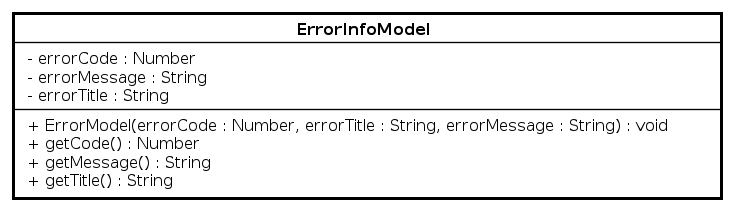
\includegraphics[scale=0.5,keepaspectratio]{UML/Classi/Front-End/QuizziPedia_Front-end_Models_ErrorInfoModel.png}
			\caption{QuizziPedia::Front-End::Models::ErrorInfoModel}
		\end{figure} \FloatBarrier
		
		\begin{itemize}
			\item \textbf{Descrizione}: rappresenta le informazioni di un errore che si è verificato eseguendo una determinata operazione;
			\item \textbf{Utilizzo}: viene utilizzata rappresentare un oggetto di tipo errore;
			\item \textbf{Relazioni con altre classi}: 
			\begin{itemize}
			 	\item \textit{OUT} \texttt{AuthService}: questa classe permette di gestire la registrazione e l'autenticazione di un utente;
			 	\item \textit{OUT} \texttt{SearchService}: questa classe permette di gestire il recupero dei dati dal back-end a seguito di una ricerca effettuata da un utente;
			 	\item \textit{OUT} \texttt{LangService}: questa classe permette di gestire la lingua nella quale si è scelto di utilizzare l'applicazione.
			 	\item \textit{OUT} \texttt{QuizService}: questa classe permette di ottenere i dati di un quiz tramite delle parole chiave inserite dall'utente nella barra di ricerca. Permette inoltre di iscriversi ad un questionario e di scaricare l'intera lista di domande di un questionario a partire dal suo id univoco;
			 	\item \textit{OUT} \texttt{StatisticsService}: questa classe permette di ottenere le statistiche dell'utente;
		 		\item \textit{OUT} \texttt{QuestionsService}: questa classe permette di ottenere domande esistenti e salvare nuove domande;
	 			\item \textit{OUT} \texttt{UserDetailsService}: questa classe permette di ottenere i dati personali degli utenti.
			\end{itemize}
			\item \textbf{Attributi}: 
			\begin{itemize}
				\item \texttt{- errorCode: Number} \\ 
				Rappresenta il codice dell'errore;
				\item \texttt{- errorMessage: String} \\ 
				Rappresenta la descrizione dell'errore; 
				\item \texttt{- errorTitle: String}\\ 
				Rappresenta il titolo del messaggio d'errore.
			\end{itemize}
			\item \textbf{Metodi}
			\begin{itemize}
				\item \texttt{+ ErrorModel(errorCode: Number, errorTitle: String, errorMessage: String) : void} \\
				Metodo costruttore della classe.\\
				\textbf{Parametri}: 
				\begin{itemize}
					\item \texttt{errorCode: Number} \\
					Parametro contenente il codice di errore;
					\item \texttt{errorTitle: String} \\
					Parametro contenente il titolo di errore;
					\item \texttt{errorMessage: String} \\
					Parametro contenente il messaggio di errore.
				\end{itemize}
				\item \texttt{+ getCode() : Number} \\
				Metodo che consente di ottenere il codice dell'errore;
				\item \texttt{+ getMessage() : String} \\
				Metodo che consente di ottenere la descrizione dell'errore;
				\item \texttt{+ getTitle() : String} \\
				Metodo che consente di ottenere il titolo del messaggio d'errore. 
			\end{itemize}
		\end{itemize}
			
		